% =====================================================================
%  FootBot — Presentación: Migración a Simulación (ROS 2 + Gazebo)
%  Beamer 16:9, compilable con pdfLaTeX (Overleaf o TeX Live).
%  Logo opcional en src/logo-unet.png. Acompaña al guion script.md (5-10 min).
% =====================================================================
\documentclass[aspectratio=169,11pt]{beamer}

\usepackage[utf8]{inputenc}
\usepackage[T1]{fontenc}
\usepackage[spanish]{babel}
\usepackage{lmodern}
\usepackage{graphicx}
\usepackage{booktabs}
\usepackage{xcolor}

% ---------- Paleta (igual que el reporte) ----------
\definecolor{unetblue}{HTML}{0B3D66}
\definecolor{accent}{HTML}{1B98A0}
\definecolor{softgray}{HTML}{F2F4F7}
\definecolor{darkgray}{HTML}{333333}

% ---------- Tema y colores ----------
\usetheme{Madrid}
\setbeamertemplate{navigation symbols}{}
\setbeamercolor{structure}{fg=unetblue}
\setbeamercolor{palette primary}{bg=unetblue,fg=white}
\setbeamercolor{palette secondary}{bg=accent,fg=white}
\setbeamercolor{palette tertiary}{bg=darkgray,fg=white}
\setbeamercolor{frametitle}{bg=unetblue,fg=white}
\setbeamercolor{title}{fg=unetblue}
\setbeamercolor{block title}{bg=accent,fg=white}
\setbeamercolor{block body}{bg=softgray}
\setbeamercolor{alerted text}{fg=accent}
\setbeamercolor{itemize item}{fg=accent}
\setbeamercolor{itemize subitem}{fg=accent}
\setbeamerfont{frametitle}{series=\bfseries}
\setbeamertemplate{itemize item}{\textbullet}
\setbeamertemplate{caption}[numbered]

\graphicspath{{figures/}{src/}}
\newcommand{\code}[1]{\texttt{\detokenize{#1}}}

% ---------- Metadatos ----------
\title[Migración a Simulación]{De la implementación física a la simulación}
\subtitle{Robot futbolista \textit{FootBot} hacia ROS\,2 Humble + Gazebo Fortress}
\author[Chacón Gómez]{Chacón Gómez, José Daniel}
\institute[UNET]{Universidad Nacional Experimental del Táchira (UNET)}
\date{Junio de 2026}

\begin{document}

% ======================= 1. PORTADA =======================
\begin{frame}[plain]
  \centering
  \vspace{0.3cm}
  \IfFileExists{src/logo-unet.png}
    {
\includegraphics[height=1.7cm]{src/logo-unet.png}\par\vspace{0.35cm}}
    {\setlength{\fboxsep}{6pt}\fbox{\parbox[c][1.1cm][c]{0.40\textwidth}{\centering\scriptsize\itshape Logo de la universidad en \texttt{src/logo-unet.png}}}\par\vspace{0.35cm}}
  {\footnotesize\textsc{Universidad Nacional Experimental del Táchira (UNET)}\par}
  \vspace{0.5cm}
  {\color{unetblue}\rule{0.9\linewidth}{1pt}}\par\vspace{0.35cm}
  {\LARGE\bfseries\color{unetblue} De la implementación física a la simulación\par}
  \vspace{0.25cm}
  {\large Migración del robot futbolista \textit{FootBot} a ROS\,2 + Gazebo\par}
  \vspace{0.25cm}
  {\color{unetblue}\rule{0.9\linewidth}{1pt}}\par
  \vspace{0.7cm}
  {\large\textbf{Chacón Gómez, José Daniel}\par}
  \vspace{0.15cm}
  {\small Proyecto FootBot / Auto Soccer Bot \;$\cdot$\; Junio de 2026\par}
\end{frame}

% ======================= 2. HOJA DE RUTA =======================
\begin{frame}{Hoja de ruta}
  \begin{columns}[T]
    \begin{column}{0.5\textwidth}
      \begin{enumerate}
        \item El punto de partida: el robot real
        \item ¿Por qué migrar a simulación?
        \item Del robot físico a ROS\,2 + Gazebo
        \item Arquitectura del sistema
      \end{enumerate}
    \end{column}
    \begin{column}{0.5\textwidth}
      \begin{enumerate}
        \setcounter{enumi}{4}
        \item Fases del trabajo
        \item Comportamientos autónomos
        \item Percepción y \emph{datasets}
        \item Resultados y trabajo futuro
      \end{enumerate}
    \end{column}
  \end{columns}
\end{frame}

% ======================= 3. PUNTO DE PARTIDA =======================
\begin{frame}{El punto de partida: el robot real}
  \begin{columns}[T]
    \begin{column}{0.58\textwidth}
      \textbf{FootBot / Auto Soccer Bot}: robot futbolista de bajo costo con \alert{ESP32-CAM}.
      \medskip

      Operaba en dos modos:
      \begin{itemize}
        \item \textbf{Manual:} control por \alert{gestos de la mano} (MediaPipe) desde el portátil.
        \item \textbf{Automático:} el ESP32-CAM transmite vídeo; el portátil detecta el balón (HSV + YOLO) y una \alert{FSM} lo sigue.
      \end{itemize}
      \medskip

      Percepción y decisión en el portátil; comandos por HTTP \code{/move}.
    \end{column}
    \begin{column}{0.42\textwidth}
      \centering
      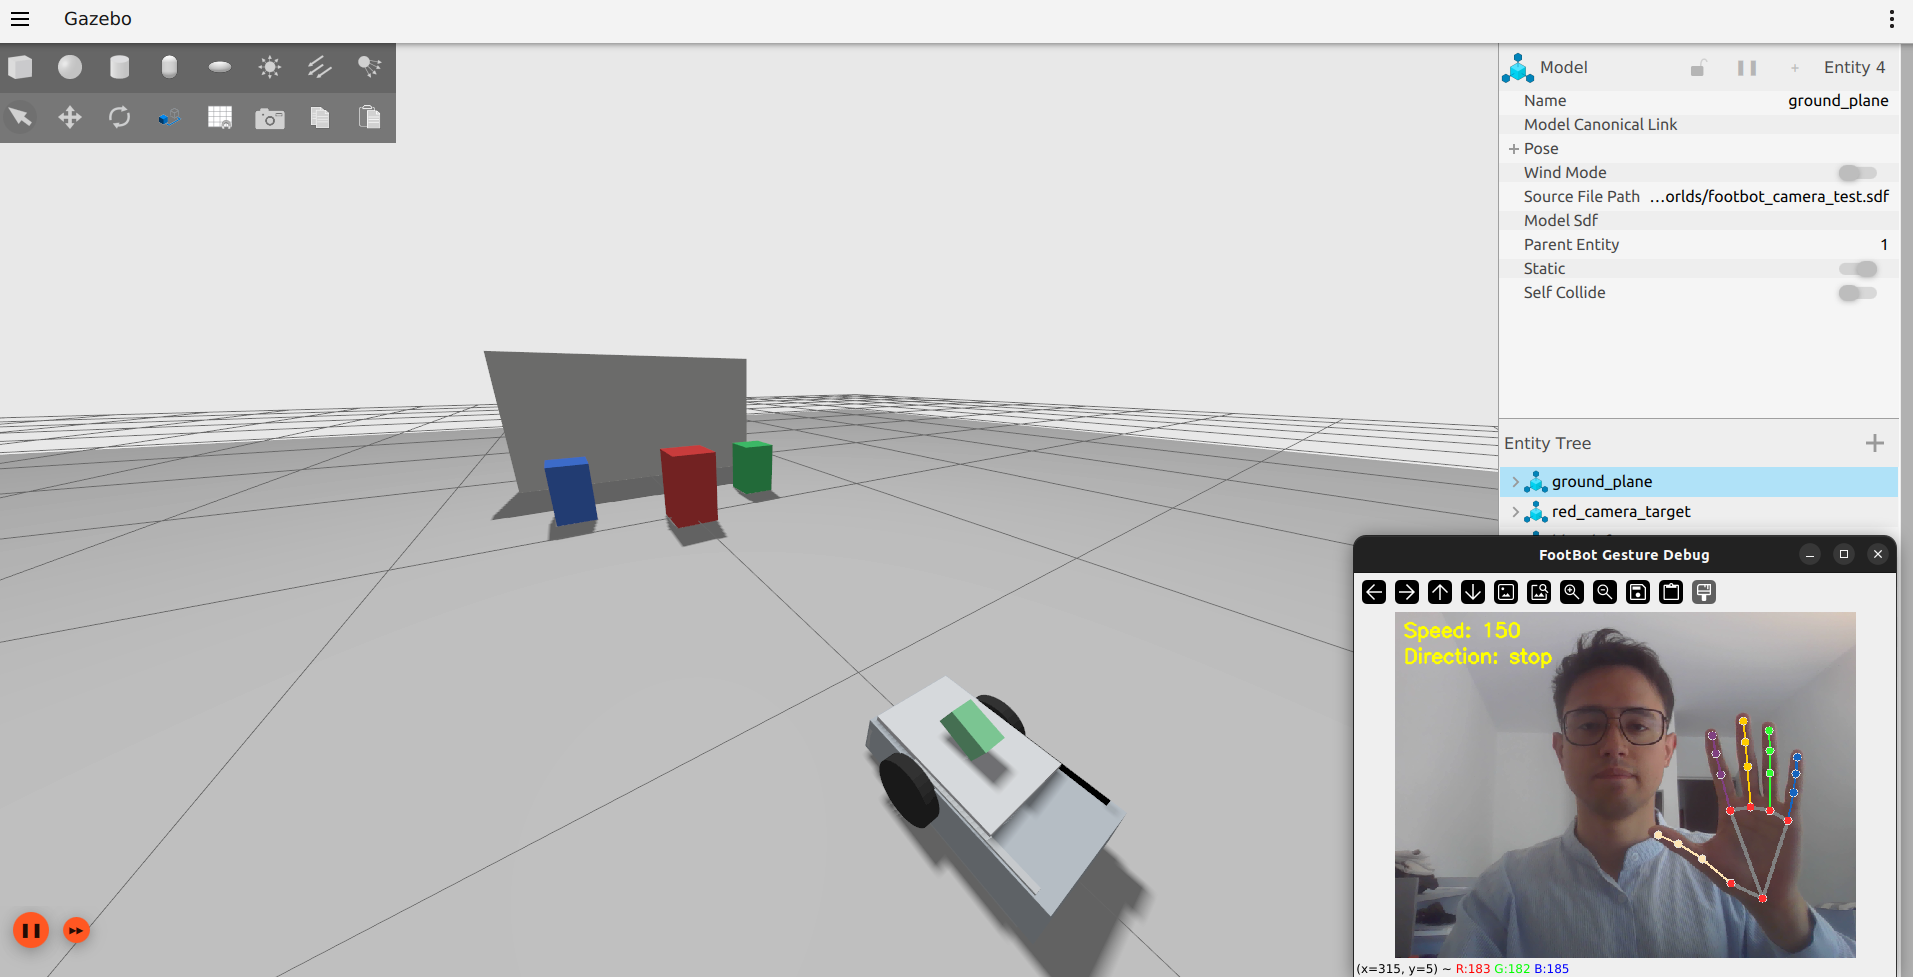
\includegraphics[width=\linewidth]{figures/gesture-debug.png}
      \par\vspace{2pt}{\scriptsize Control por gestos con MediaPipe.}
    \end{column}
  \end{columns}
\end{frame}

% ======================= 4. MOTIVACIÓN =======================
\begin{frame}{¿Por qué migrar a simulación?}
  \begin{columns}[T]
    \begin{column}{0.5\textwidth}
      \textbf{Límites del banco físico}
      \begin{itemize}
        \item Hardware frágil y costoso
        \item Dependencia de la iluminación
        \item Un solo robot, iteración lenta
      \end{itemize}
    \end{column}
    \begin{column}{0.5\textwidth}
      \textbf{Ventajas de la simulación}
      \begin{itemize}
        \item Reproducible y determinista
        \item Segura y sin costo por iterar
        \item Escenarios en paralelo
        \item Base para comportamientos avanzados
      \end{itemize}
    \end{column}
  \end{columns}
  \vspace{0.35cm}
  \begin{block}{Principio}
    No se desecha lo anterior: el robot ESP32 queda como \alert{referencia} y su protocolo HTTP \code{/move} se conserva mediante un puente.
  \end{block}
\end{frame}

% ======================= 5. MAPEO FÍSICO -> SIMULACIÓN =======================
\begin{frame}{Del robot físico al entorno simulado}
  \centering
  \renewcommand{\arraystretch}{1.25}
  \footnotesize
  \begin{tabular}{ll}
    \toprule
    \textbf{Robot físico (ESP32)} & \textbf{Simulación (ROS\,2 + Gazebo)} \\
    \midrule
    Tracción diferencial + L298N & Modelo URDF/Xacro + plugin DiffDrive \\
    Cámara ESP32-CAM (MJPEG) & Cámara de Gazebo $\rightarrow$ \code{/camera/image_raw} \\
    API HTTP \code{/move} & \code{footbot_bridge} $\rightarrow$ \code{/cmd_vel} \\
    Visión en el portátil (HSV/YOLO) & \code{footbot_perception} / \code{footbot_soccer_vision} \\
    FSM de seguimiento & \code{footbot_soccer_behavior} (FSM) \\
    \bottomrule
  \end{tabular}

  \vspace{0.35cm}
  \normalsize Estrategia \alert{\emph{simulation-first}}: reconstruir cada capacidad como paquetes de ROS\,2, reutilizando los conceptos del robot real.
\end{frame}

% ======================= 6. ARQUITECTURA =======================
\begin{frame}{Arquitectura del sistema de simulación}
  \begin{columns}[T]
    \begin{column}{0.54\textwidth}
      \textbf{Stack}
      \begin{itemize}
        \item ROS\,2 Humble + Gazebo Fortress
        \item Integración \code{ros_gz} (puente ROS\,$\leftrightarrow$\,Gazebo)
      \end{itemize}
      \medskip

      \textbf{Flujo de datos}
      \begin{itemize}
        \item Gazebo $\rightarrow$ \code{ros_gz_bridge} $\rightarrow$ topics
        \item Percepción $\rightarrow$ estado $\rightarrow$ FSM $\rightarrow$ \code{/cmd_vel}
      \end{itemize}
      \medskip

      \alert{Regla de oro:} un solo nodo dueño de \code{/cmd_vel}.
    \end{column}
    \begin{column}{0.46\textwidth}
      \centering
      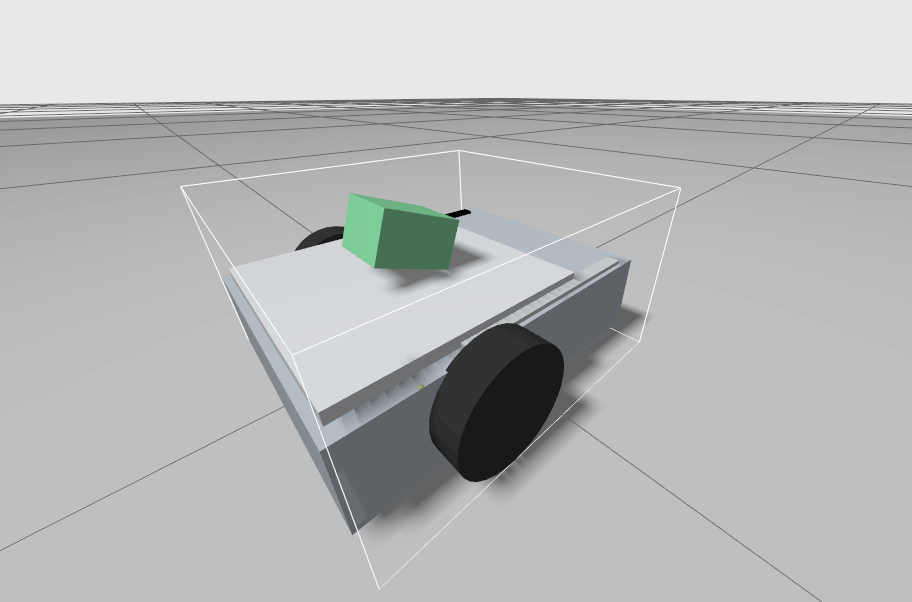
\includegraphics[width=\linewidth]{figures/simulation-overview.png}
      \par\vspace{2pt}{\scriptsize FootBot en Gazebo con su cámara simulada.}
    \end{column}
  \end{columns}
\end{frame}

% ======================= 7. FASES =======================
\begin{frame}{Fases del trabajo realizado}
  \begin{enumerate}
    \item \textbf{Fundamentos:} modelo del robot (URDF/Xacro), mundos y arranque en Gazebo.
    \item \textbf{Puentes de control:} \code{/cmd_vel}, puente HTTP \code{/move} (ESP32) y gestos nativos en ROS.
    \item \textbf{Percepción simulada:} cámara del robot, detección HSV del balón y visión YOLO.
    \item \textbf{Comportamientos autónomos:} \emph{Control de balón} y \emph{Llegar a la portería}, deterministas por FSM.
    \item \textbf{Datasets y entrenamiento:} captura, etiquetado, aumento y entrenamiento de YOLO.
  \end{enumerate}
\end{frame}

% ======================= 8. CONTROL DE BALÓN =======================
\begin{frame}{Comportamiento 1: Control de balón}
  \begin{columns}[T]
    \begin{column}{0.55\textwidth}
      Encontrar, aproximarse, contactar y \alert{mantener} el balón en una zona de control frontal.
      \medskip
      \begin{itemize}
        \item Detección HSV $\rightarrow$ \code{BallState}
        \item FSM: buscar, alinear, aproximar, contactar, controlar, recuperar, parada segura
        \item Las \emph{skills} solo producen comandos \code{Twist} acotados; la FSM decide las transiciones.
      \end{itemize}
    \end{column}
    \begin{column}{0.45\textwidth}
      \centering
      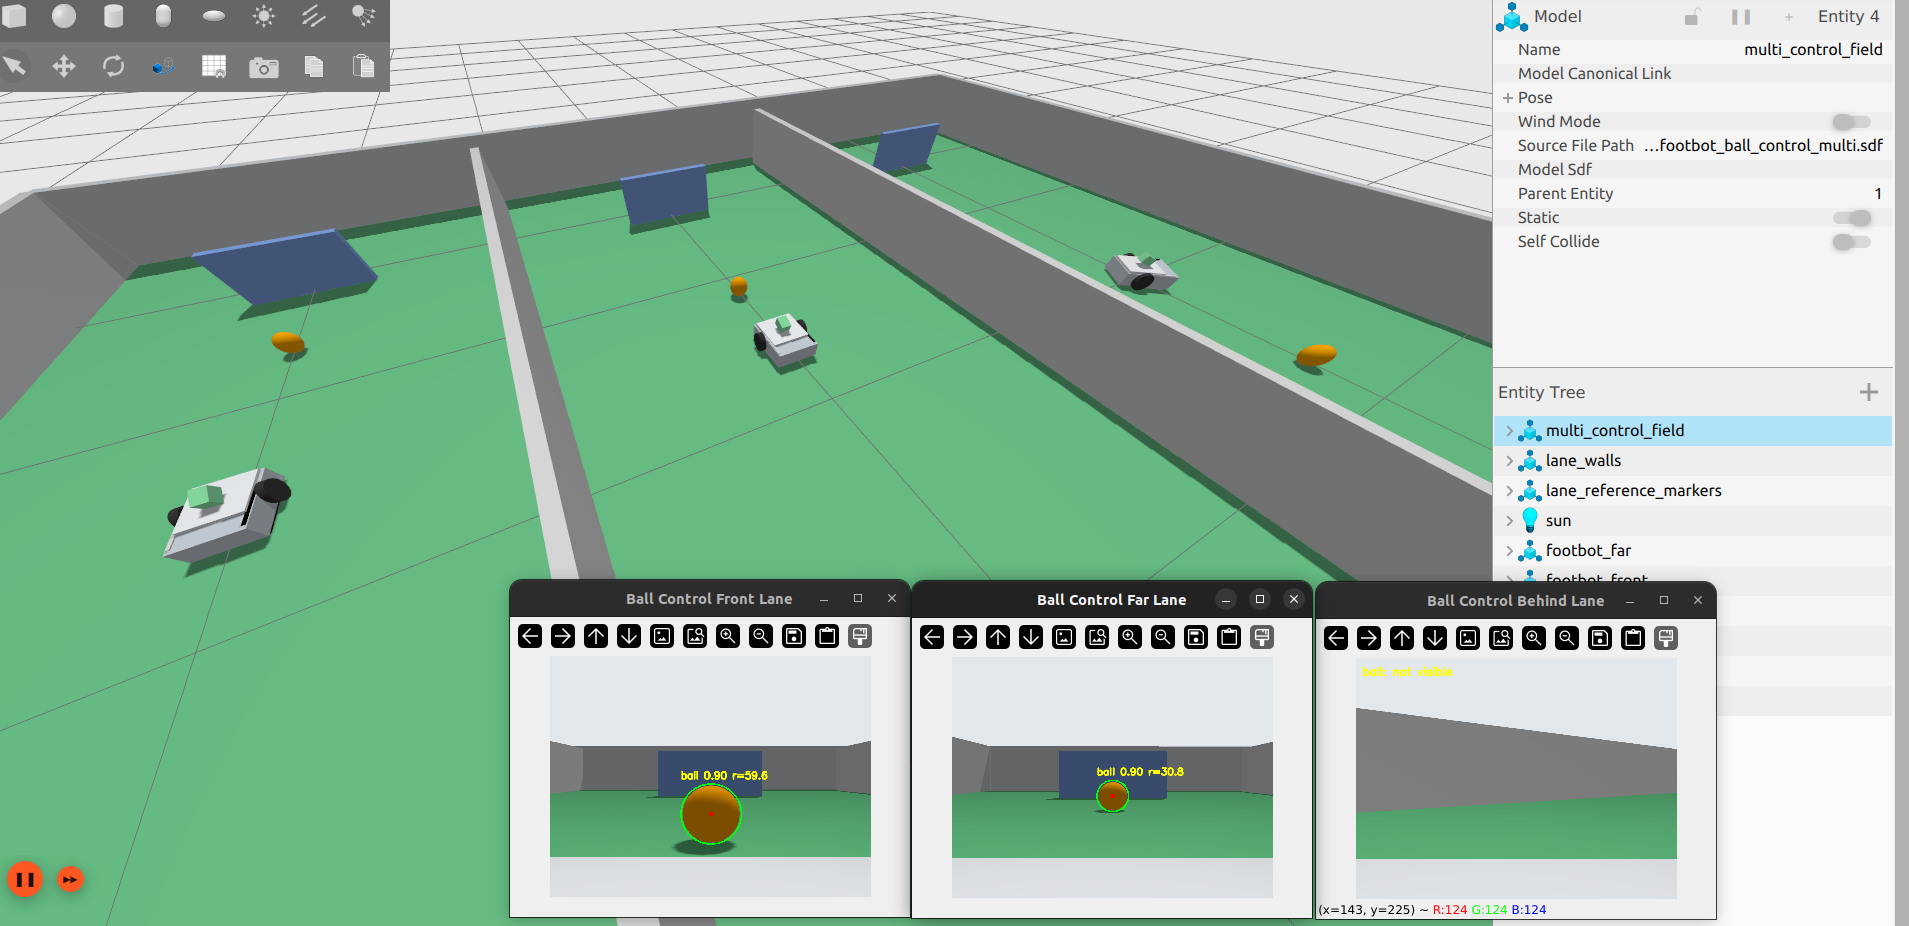
\includegraphics[width=\linewidth]{figures/ball-control-debug.png}
      \par\vspace{2pt}{\scriptsize Depuración: balón detectado y estado.}
    \end{column}
  \end{columns}
\end{frame}

% ======================= 8b. CONTROL DE BALÓN: FORMULACIÓN =======================
\begin{frame}{Control de balón: ¿cómo lo mantiene centrado?}
  \textbf{Idea:} el robot \alert{solo ve el balón en la imagen}; ``centrado'' = el balón en el centro del cuadro. Mide cuánto se desvía y gira para corregirlo.
  \medskip

  \textbf{1. Mide la desviación} como un ángulo $\theta$ (si está centrado, $\theta = 0$):
  \[ \theta = \arctan\!\left(\frac{u - W/2}{f}\right) \]

  \textbf{2. Gira proporcional al error} (más descentrado $\Rightarrow$ corrige más rápido):
  \[ \omega = -\,K_p\,\theta \qquad (\text{el signo} - \text{ gira hacia el balón}) \]

  \textbf{3. Lo da por ``controlado''} solo si sigue centrado y cerca un tiempo:
  \[ \lvert\theta\rvert \le \theta_{\mathrm{tol}} \ \text{ y }\ d \le d_{\mathrm{ctrl}} \ \text{ durante } \ge T_{\mathrm{hold}} \]
\end{frame}

% ======================= 9. LLEGAR A LA PORTERÍA =======================
\begin{frame}{Comportamiento 2: Llegar a la portería}
  Empujar el balón hacia una portería visible, \alert{guiado solo por percepción} (sin usar poses reales de Gazebo).
  \medskip
  \begin{itemize}
    \item Detector YOLO de \code{ball} + \code{goal} $\rightarrow$ \code{BallGoalState}.
    \item FSM: buscar balón, controlarlo, buscar/alinear portería, driblar y marcar.
    \item \textbf{Memoria temporal de la portería} cuando desaparece a corta distancia.
    \item \code{COMMIT_TO_GOAL}: empuje final lento, centrado en el balón.
    \item Un \textbf{árbitro de simulación} detecta el gol y detiene el episodio.
  \end{itemize}
\end{frame}

% ======================= 10. PERCEPCIÓN Y DATASETS =======================
\begin{frame}{Percepción y \emph{datasets}}
  \begin{columns}[T]
    \begin{column}{0.55\textwidth}
      \textbf{Detección}
      \begin{itemize}
        \item Cámara $\rightarrow$ \code{/camera/image_raw}
        \item HSV (balón) + YOLO (balón, portería, oponente)
      \end{itemize}
      \medskip

      \textbf{Tubería de datos (YOLO)}
      \begin{itemize}
        \item Captura $\rightarrow$ etiquetado en Label Studio
        \item Aumento $\rightarrow$ validación $\rightarrow$ entrenamiento
      \end{itemize}
    \end{column}
    \begin{column}{0.45\textwidth}
      \centering
      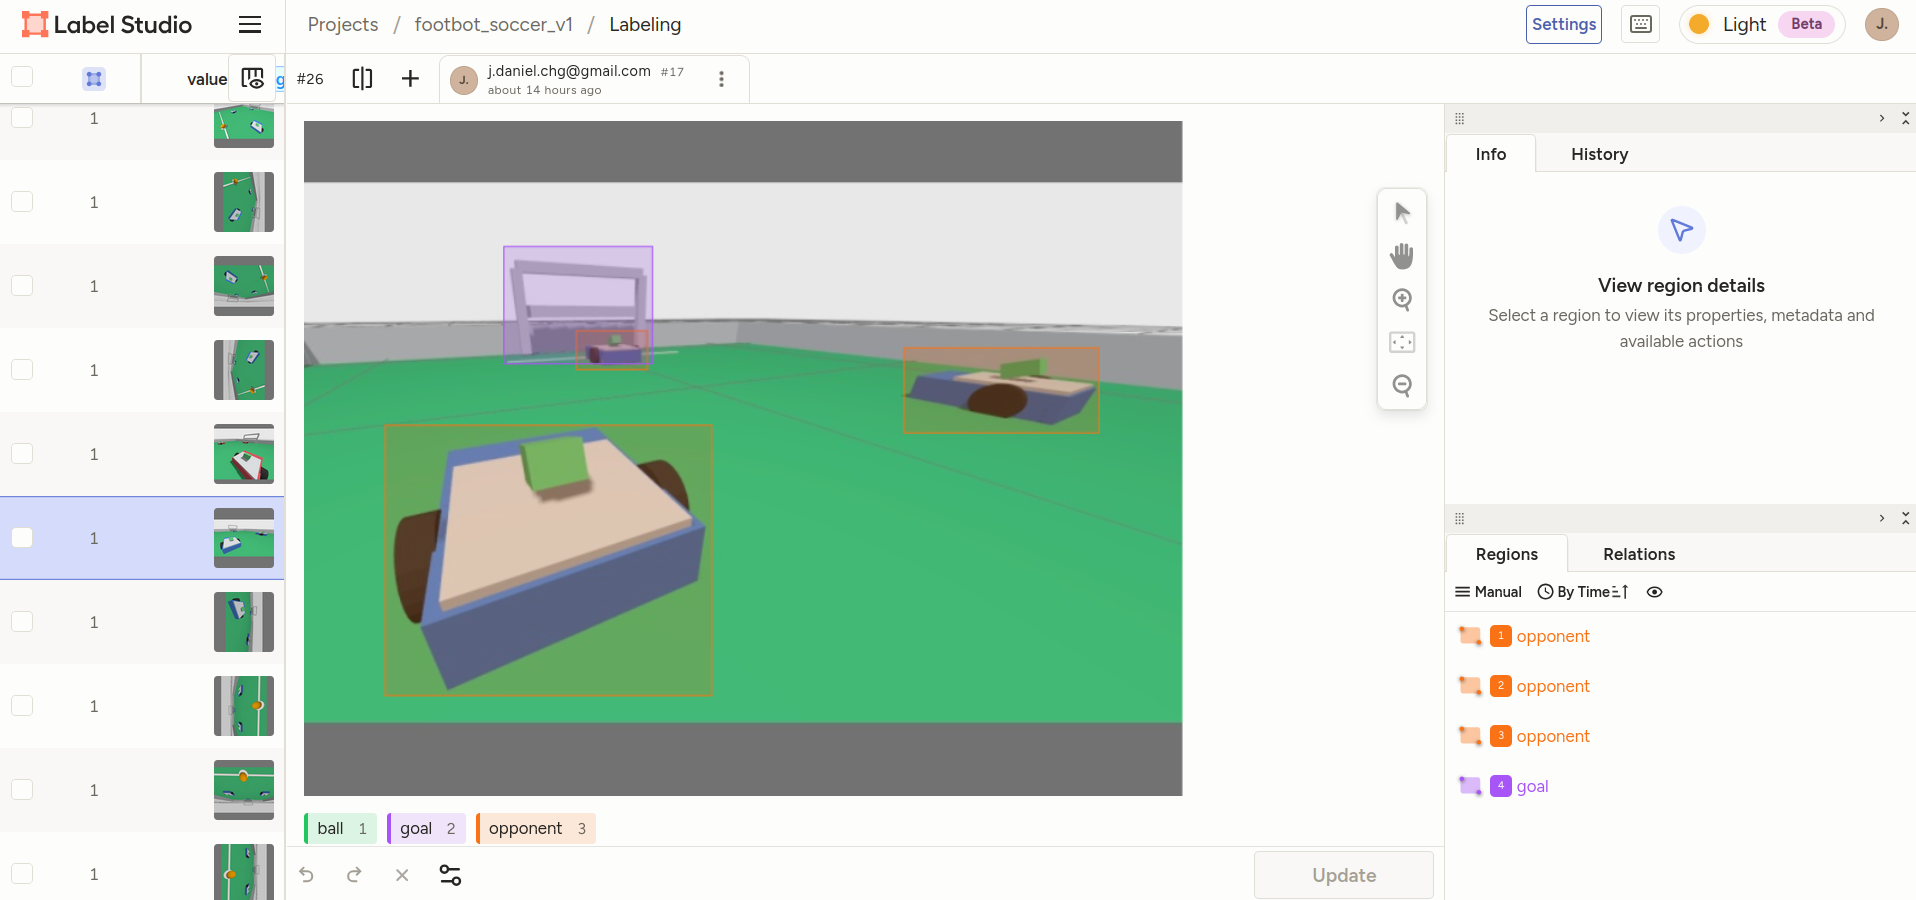
\includegraphics[width=\linewidth]{figures/yolo-labeling.png}
      \par\vspace{2pt}{\scriptsize Etiquetado de objetos en Label Studio.}
    \end{column}
  \end{columns}
\end{frame}

% ======================= 11. RESULTADOS =======================
\begin{frame}{Resultados y estado actual}
  \begin{columns}[T]
    \begin{column}{0.56\textwidth}
      \textbf{Implementado y funcionando:}
      \begin{itemize}
        \item Robot, mundos y movimiento por \code{/cmd_vel}
        \item Puente HTTP \code{/move} y gestos en ROS
        \item Control de balón y Llegar a la portería
        \item Herramientas de \emph{dataset} y entrenamiento YOLO
      \end{itemize}
      \medskip

      \alert{Verificación:} la suite de \code{footbot_soccer_behavior} pasa (41 pruebas, 0 fallos).
    \end{column}
    \begin{column}{0.44\textwidth}
      \centering
      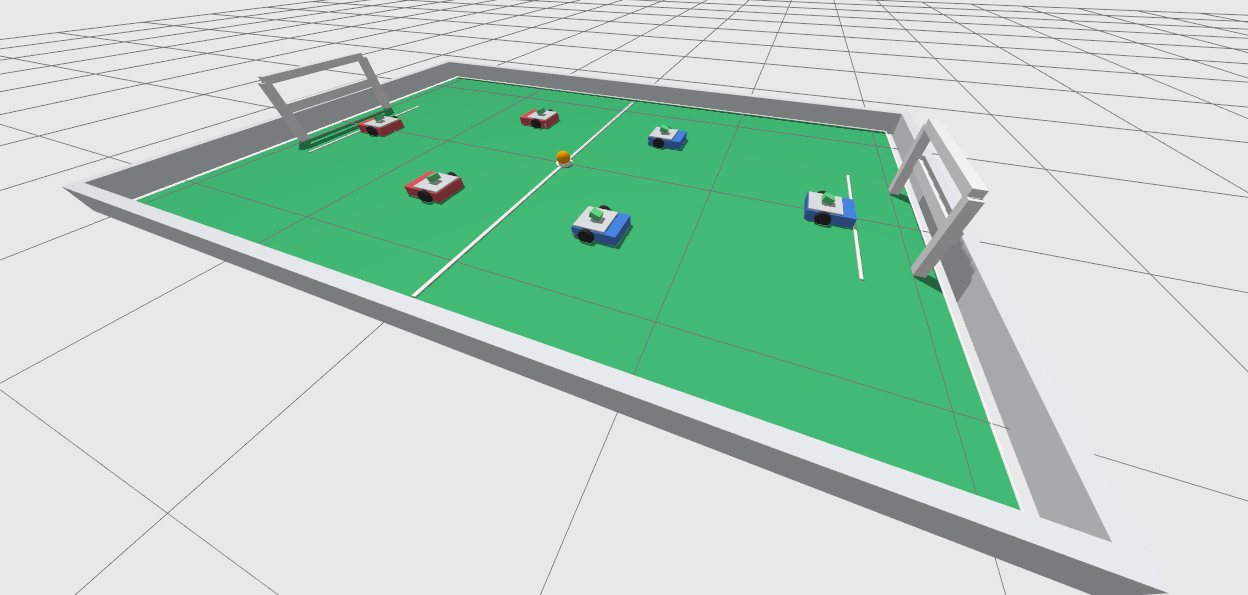
\includegraphics[width=\linewidth]{figures/soccer-field.png}
      \par\vspace{2pt}{\scriptsize Campo de fútbol completo.}
    \end{column}
  \end{columns}
\end{frame}

% ======================= 11b. RESULTADO CLAVE: REMATE A CORTA DISTANCIA =======================
\begin{frame}{Resultado clave: el remate a corta distancia}
  \begin{columns}[c]
    \begin{column}{0.40\textwidth}
      \footnotesize
      Tanda de \alert{5 episodios} de \emph{Llegar a la portería}:
      \begin{itemize}
        \item Controla el balón rápido ($\approx$9 s) y estable.
        \item Pero \alert{solo 1 de 5 marcó} (20\,\%); ese tardó $\approx$269 s.
        \item Robot y balón se \alert{estancan frente a la portería}.
      \end{itemize}
      \smallskip

      \textbf{Causa:} muy cerca, la portería \alert{no cabe en el cuadro} y YOLO no la detecta de forma continua $\Rightarrow$ la FSM pierde la referencia y reincide en \code{RECOVER_BALL} ($\approx$33\,\% del tiempo). El respaldo \code{COMMIT_TO_GOAL} \alert{no se activó} en ningún episodio.
    \end{column}
    \begin{column}{0.60\textwidth}
      \centering
      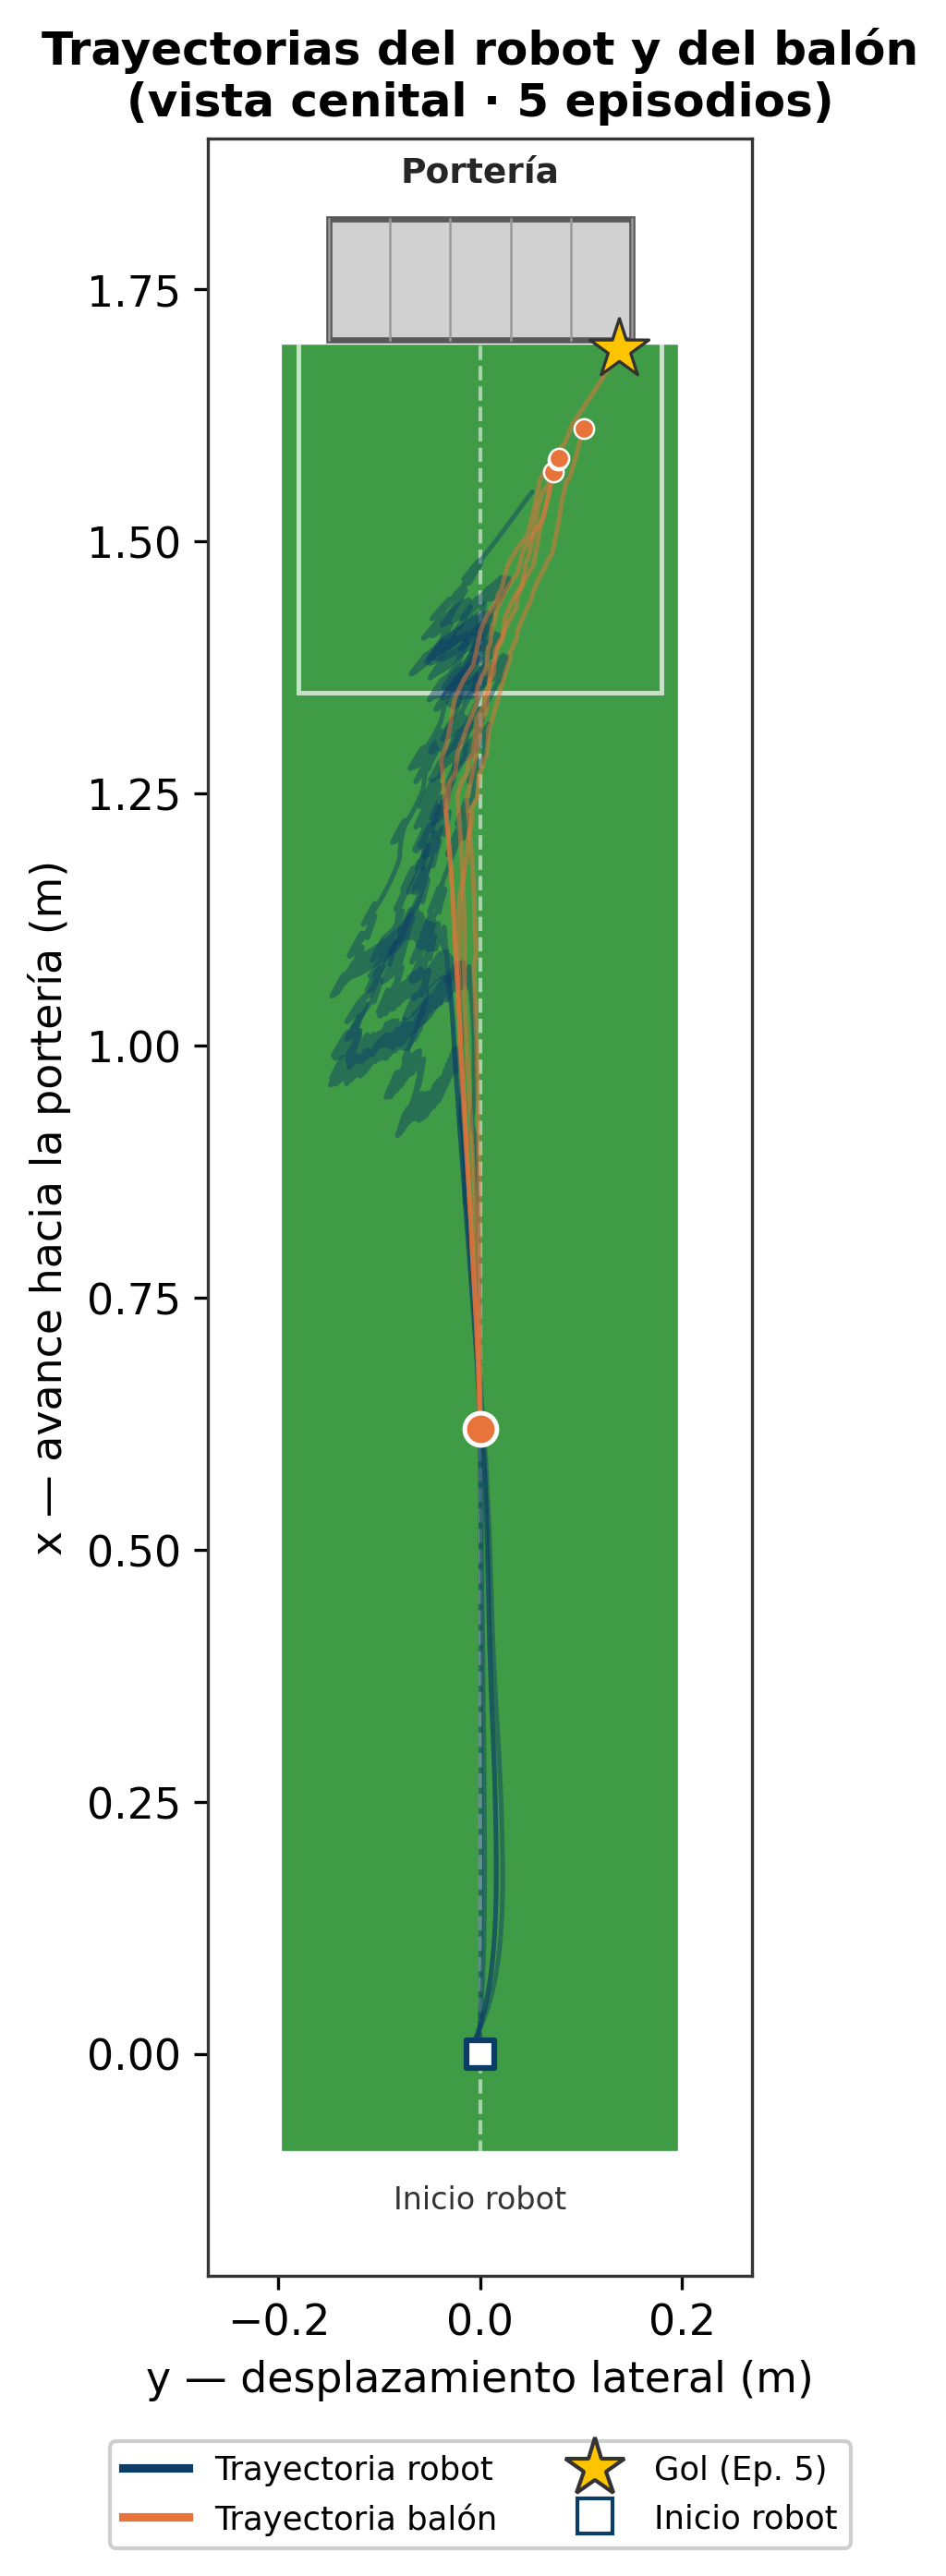
\includegraphics[height=4.7cm]{figures/trajectory_xy_vertical.png}\hfill
      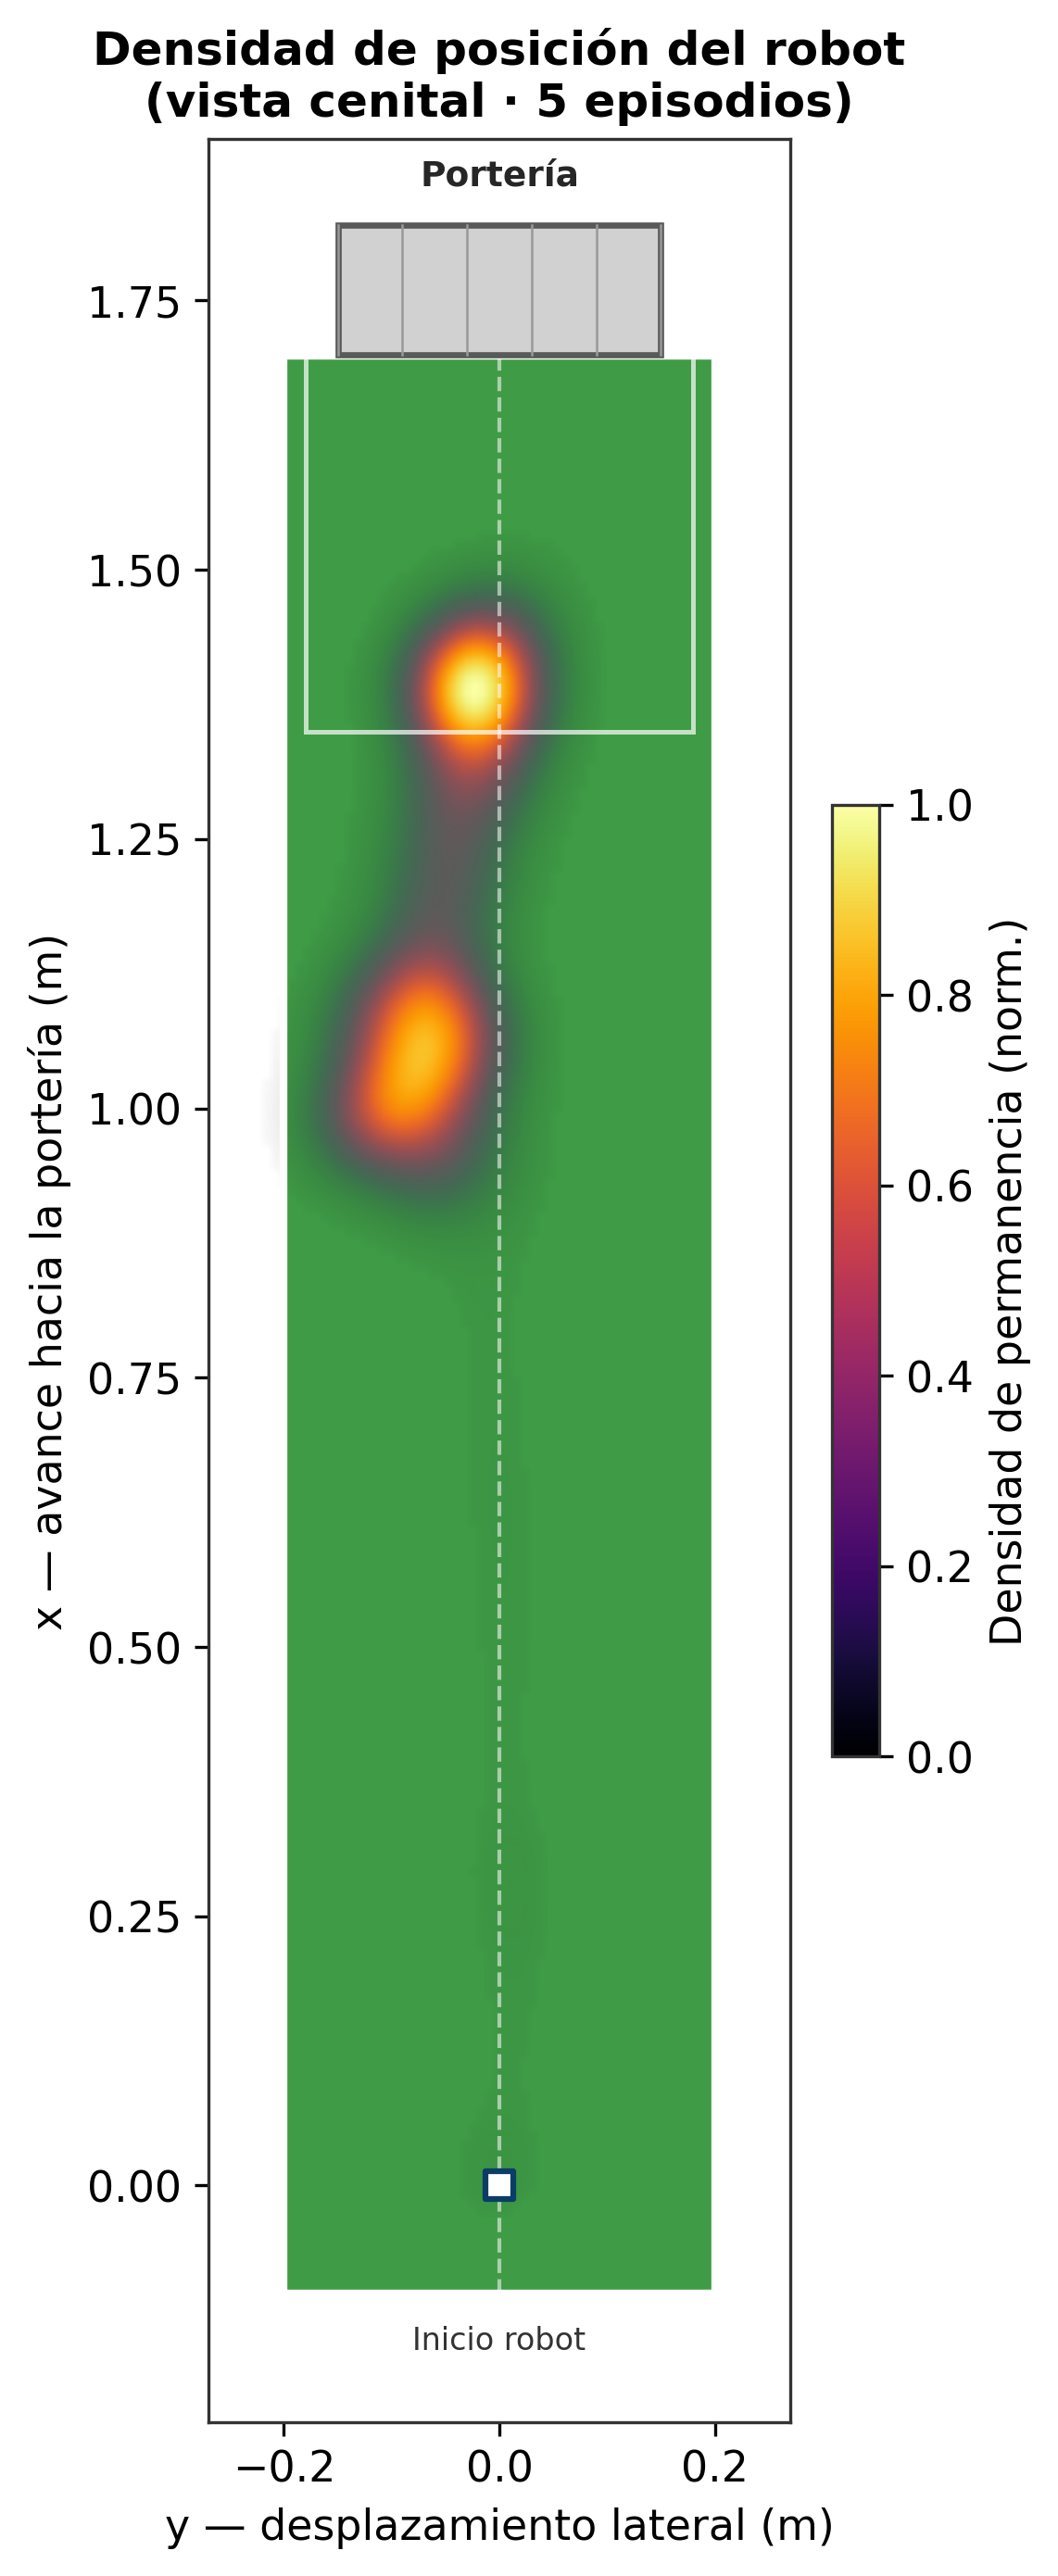
\includegraphics[height=4.7cm]{figures/robot_heatmap_vertical.png}\hfill
      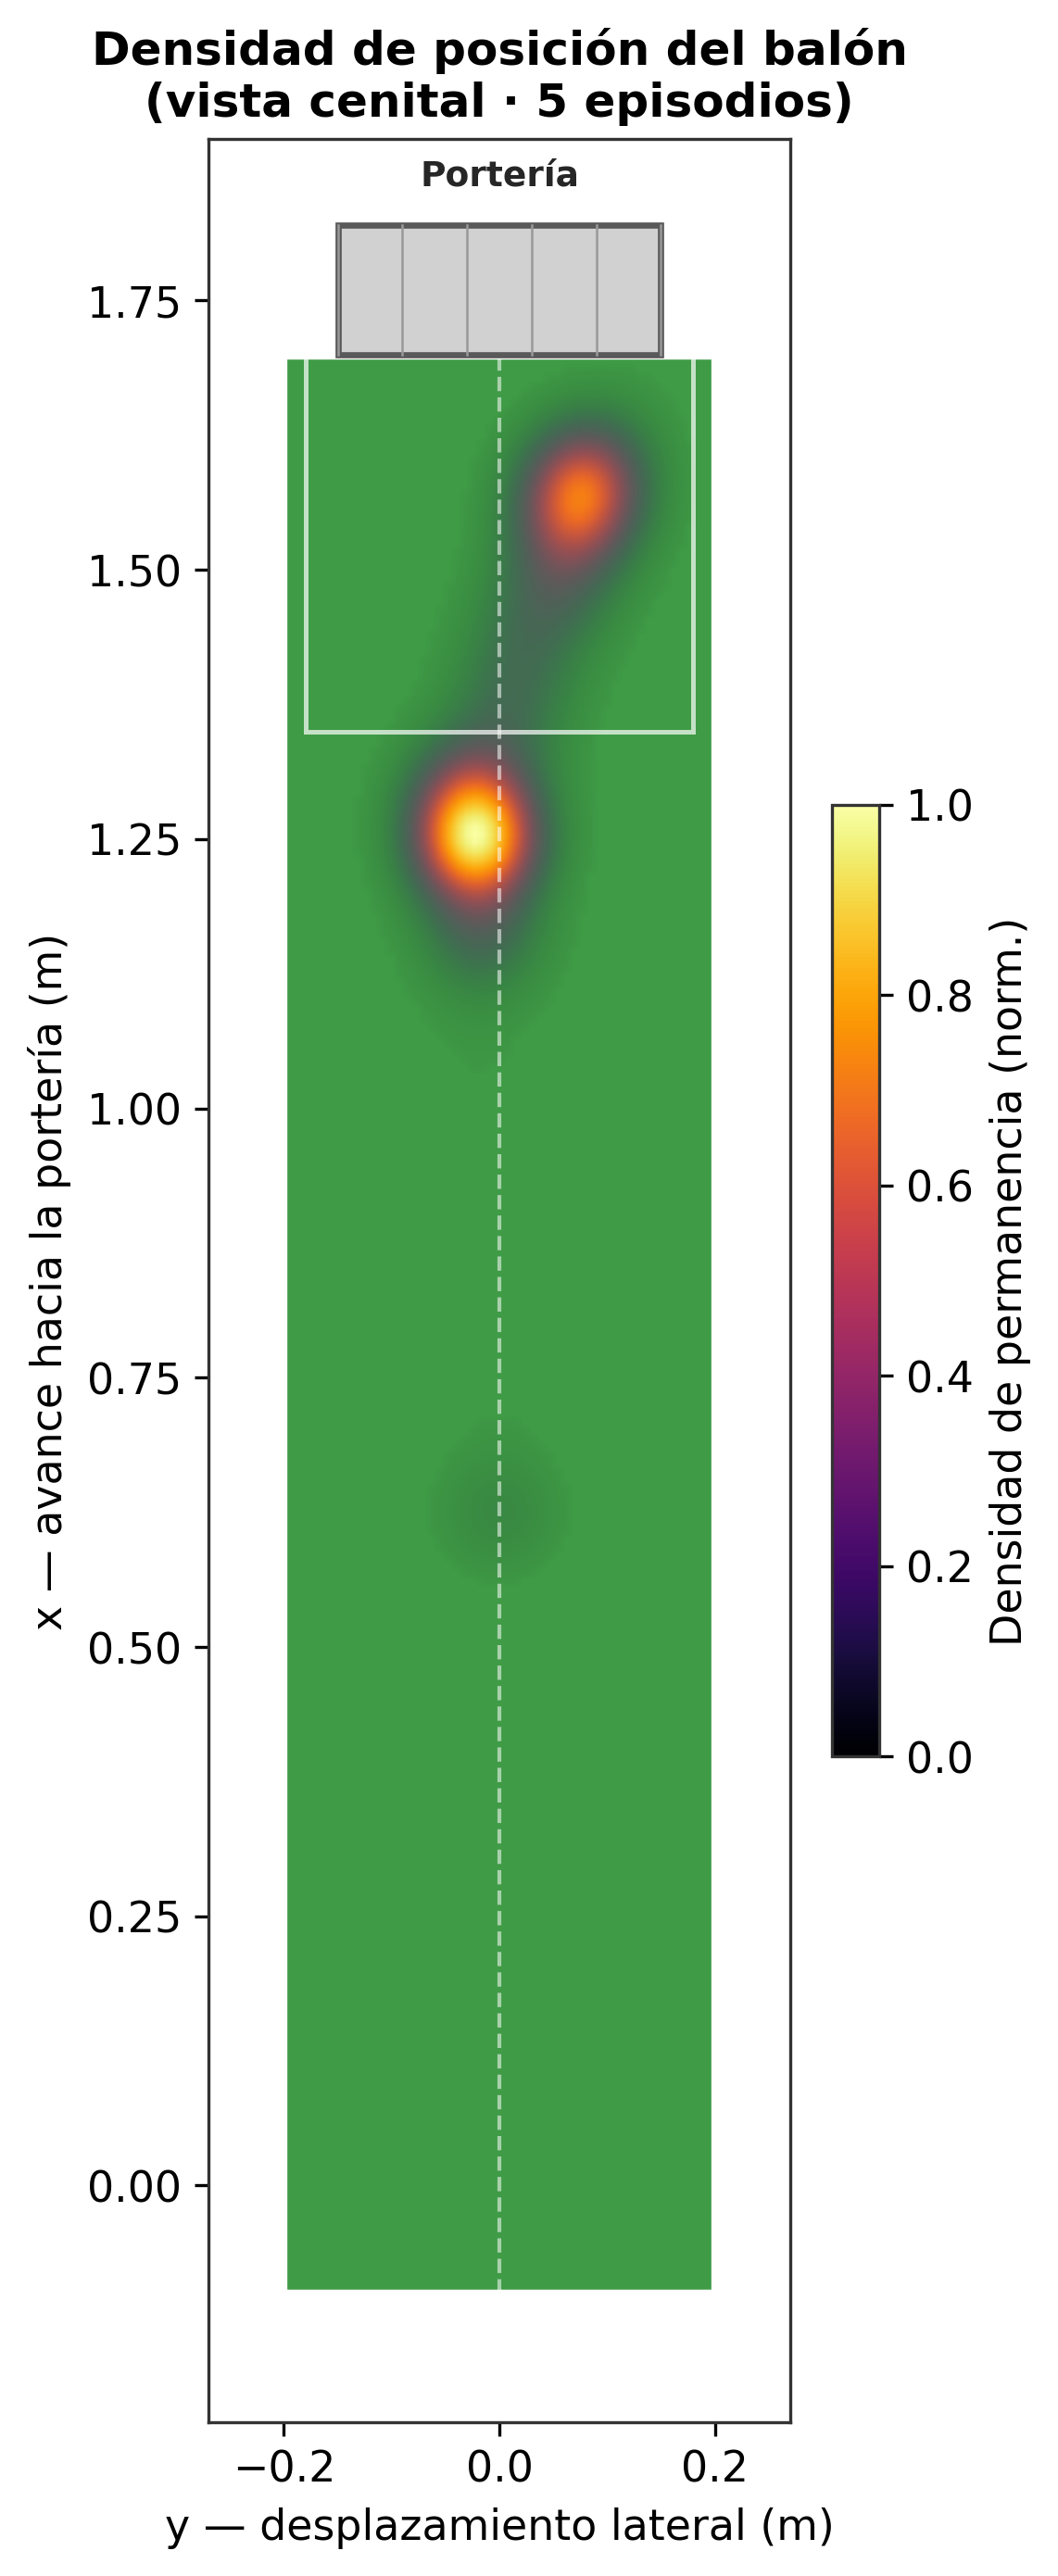
\includegraphics[height=4.7cm]{figures/ball_heatmap_vertical.png}
      \par\vspace{3pt}
      {\scriptsize (a) Trayectorias \quad (b) Densidad robot \quad (c) Densidad balón \;—\; vista cenital, portería arriba.}
    \end{column}
  \end{columns}
\end{frame}

% ======================= 12. TRABAJO FUTURO =======================
\begin{frame}{Trabajo futuro}
  \begin{itemize}
    \item \textbf{Portería a corta distancia (prioritario):} \emph{dataset} de portería cercana/parcial y reentrenar YOLO, detectar postes/línea de meta, cámara de mayor FOV, o activar el \emph{modo de remate} \code{COMMIT_TO_GOAL} guiado por la última pose\,+\,odometría.
    \item \textbf{Oponentes:} detectar y disputar el balón sin desestabilizar la base.
    \item \textbf{Juego en equipo:} tres robots por bando, con roles y \emph{namespaces} por robot.
    \item \textbf{Investigación:} árboles de comportamiento, planificación y, con métricas estables, RL/MARL.
  \end{itemize}
  \vspace{0.25cm}
  \begin{block}{Principio rector}
    Mantener la base \alert{determinista} y medible; añadir táctica solo cuando aporte y sea depurable.
  \end{block}
\end{frame}

% ======================= 13. CONCLUSIONES =======================
\begin{frame}{Conclusiones}
  \begin{itemize}
    \item La migración convirtió un banco físico frágil en un entorno \alert{reproducible, seguro y escalable}.
    \item Sin desechar lo previo: el robot ESP32 sigue como referencia.
    \item Dos comportamientos de fútbol deterministas sobre un patrón claro:\\ percepción $\rightarrow$ estado $\rightarrow$ FSM $\rightarrow$ \code{/cmd_vel}.
    \item Base sólida para oponentes, juego en equipo y experimentos tácticos.
  \end{itemize}
\end{frame}

% ======================= 14. CIERRE =======================
\begin{frame}[plain]
  \centering
  \vspace{1.1cm}
  {\color{unetblue}\rule{0.7\linewidth}{1pt}}\par\vspace{0.5cm}
  {\Huge\bfseries\color{unetblue} ¡Gracias!\par}
  \vspace{0.3cm}
  {\large Preguntas y comentarios\par}
  \vspace{0.4cm}
  {\color{unetblue}\rule{0.7\linewidth}{1pt}}\par
  \vspace{0.6cm}
  {\small Chacón Gómez, José Daniel \;$\cdot$\; UNET \;$\cdot$\; Proyecto FootBot\par}
\end{frame}

\end{document}
